\section{Problem Set 7}

\subsection{Recap of Relative Orbital Work}

\subsection{Initial Navigation System Design}

\subsubsection{Choice of State Representation}
We will be using an Extended Kalman Filter (EKF) for our navigation system. Within the EKF, we will use a mixed state representation of absolute and relative orbit elements of the chief and deputies. Specifically, we will estimate the absolute orbit elements of the chief and the relative orbit elements of the deputy. The resulting state vector is:

\begin{equation}
\begin{bmatrix}
\boldsymbol{\alpha}_1 \\
\hline
\delta \boldsymbol{\alpha}_2 \\
\hline
\delta \boldsymbol{\alpha}_3
\end{bmatrix}
=
\begin{bmatrix}
a_1 \\
e_{x,1} \\
e_{y,1} \\
i_1 \\
\Omega_1 \\
u_1 \\
\hline
\delta a_2 \\
\delta \lambda_2 \\
\delta e_{x,2} \\
\delta e_{y,2} \\
\delta i_{x,2} \\
\delta i_{y,2} \\
\hline
\delta a_3 \\
\delta \lambda_3 \\
\delta e_{x,3} \\
\delta e_{y,3} \\
\delta i_{x,3} \\
\delta i_{y,3}
\end{bmatrix}
\end{equation}

This state representation was chosen because we are not assuming perfect knowledge of the absolute chief state, so we must estimate it. This estimated absolute chief state then informs our estimation of the relative states of the deputies, which are inherently the focus of our docking and servicing mission. Orbit elements in general were chosen because they give more immediately intuitive understandings of the relative state and change much less rapidly then Cartesian position and velocity do. This makes it easier for our filter to accurate estimate the state since the magnitude of propagation steps is smaller. 

\subsubsection{Dynamics Model for State Prediction}
For predicting the state within the filter, two different dynamics models will be used. For predicting the absolute chief orbit elements, the nonlinear Gauss Variational Equations (GVEs) will be numerically integrated. This approach is outlined in Section \ref{{sec:osc_mean_J2}}. For predicting the relative orbit elements of the deputies, the ROEs will be propagated via numerical integration of the following expression from Koenig \cite{koenig2017new}:

\begin{equation}
\delta \dot{\boldsymbol{\alpha}_{\text{qns}'}} = 
\kappa_d
\begin{pmatrix}
0 \\
\eta_d(3\cos^2 i_d - 1) + (5\cos^2 i_d - 1) - 2\cos i_d \cos i_c \\
- e_d \sin(\omega_d - \omega_c)(5\cos^2 i_d - 1) \\
e_d \cos(\omega_d - \omega_c)(5\cos^2 i_d - 1) \\
0 \\
-2\cos i_d \sin i_c
\end{pmatrix}
-
\kappa_c
\begin{pmatrix}
0 \\
(1 + \eta_c)(3\cos^2 i_c - 1) \\
- e_d \sin(\omega_d - \omega_c)(5\cos^2 i_c - 1) \\
e_d \cos(\omega_d - \omega_c)(5\cos^2 i_c - 1) \\
0 \\
-2\cos i_c \sin i_c \\
\end{pmatrix}
\tag{23}
\end{equation}

where
\begin{align*}
\eta_d &= \sqrt{1 - e_d^2} \\
\eta_c &= \sqrt{1 - e_c^2} \\
\\
\kappa_d &= \frac{3 J_2 R_E^2 \sqrt{\mu}}{4 a_d^{7/2} \eta_d^4} \\
\kappa_c &= \frac{3 J_2 R_E^2 \sqrt{\mu}}{4 a_c^{7/2} \eta_c^4}
\end{align*}

This expression is the time derivative of the 


Note that

\begin{equation}
\delta \boldsymbol{\alpha}_{\text{qns}'} = \mathbf{J}_{\text{qns}}(\alpha_c) \, \delta \boldsymbol{\alpha}_{\text{qns}}
\end{equation}

\begin{equation}
\mathbf{J}_{\text{qns}}(\alpha_c) =
\begin{bmatrix}
\mathbf{I}_{2 \times 2} & \mathbf{0}_{2 \times 2} & \mathbf{0}_{2 \times 2} \\
\mathbf{0}_{2 \times 2} & 
\begin{bmatrix}
\cos \omega & \sin \omega \\
-\sin \omega & \cos \omega
\end{bmatrix}
& \mathbf{0}_{2 \times 2} \\
\mathbf{0}_{2 \times 2} & \mathbf{0}_{2 \times 2} & \mathbf{I}_{2 \times 2}
\end{bmatrix}
\end{equation}

\begin{equation}
\delta \boldsymbol{\alpha}_{\text{qns}'} =
\begin{pmatrix}
\delta a \\
\delta \lambda \\
\delta e_{x'} \\
\delta e_{y'} \\
\delta i_x \\
\delta i_y
\end{pmatrix}
=
\begin{pmatrix}
\frac{a_d - a_c}{a_c} \\
(M_d - M_c) + (\omega_d - \omega_c) + (\Omega_d - \Omega_c) \cos i_c \\
e_d \cos(\omega_d - \omega_c) - e_c \\
e_d \sin(\omega_d - \omega_c) \\
i_d - i_c \\
(\Omega_d - \Omega_c) \sin i_c
\end{pmatrix}
\end{equation}

The control input matrix is defined by Chernick as \cite{chernick2021optimal}:
\begin{equation}
\Delta \delta \boldsymbol{\alpha}_k = \boldsymbol{\Gamma}_k \delta \mathbf{v}_k = 
\frac{1}{n a}
\begin{bmatrix}
0 & 2 & 0 \\
-2 & 0 & 0 \\
\sin(u_k) & 2 \cos(u_k) & 0 \\
-\cos(u_k) & 2 \sin(u_k) & 0 \\
0 & 0 & \cos(u_k) \\
0 & 0 & \sin(u_k)
\end{bmatrix}
\begin{bmatrix}
\delta v_R \\
\delta v_T \\
\delta v_N
\end{bmatrix}
\end{equation}



The filter uses Euler integration as opposed to Runge Kutta integration so to be computationally less expensive and provide more distinction from the ground truth. 

\begin{figure}[H]
    \centering
    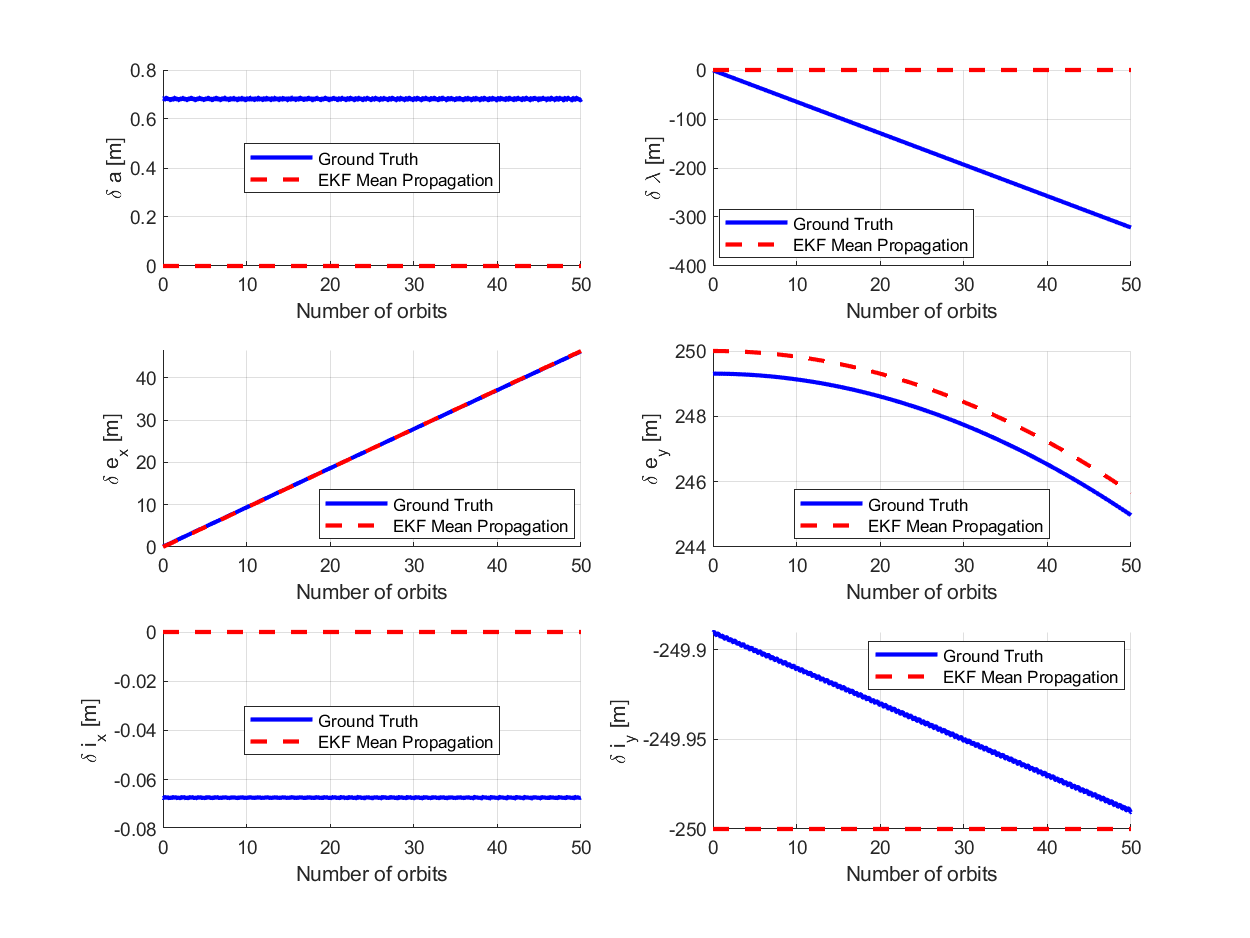
\includegraphics[width=0.75\linewidth]{sim/figures/PS7/ROE_over_time_SV3_comparison.png}
    \caption{ROE over time comparison for SV3}
    \label{fig:enter-label}
\end{figure}

\subsubsection{Linearized Dynamics Model for Covariance Update}

\subsubsection{On-board Sensors and Measurements}

Each of the deputies (SV2 and SV3) is equipped with the following sensors, which also give the raw measurements mentioned below:
\begin{itemize}
    \item \textbf{Vision-based sensors:} These provide relative bearing angle measurements for SV2 and SV3 relative to SV1. We assume that the sensors on SV2 and SV3 are always pointed at SV1. For close-range measurements required during SV3's docking phase, the vision-based sensors can also provide feature-rich images that may be used for more accurate position estimation. 
    \item \textbf{GNSS antennas:} These provide GNSS measurements such as pseudoranges. For simplicity, we stick with the single-difference GNSS pseudoranges. Although, in the future, we will consider combing the pseudo-range measurements get to apply double-difference GNSS methods.
\end{itemize}

These raw measurements can be converted into useful pseudo-measurements based on standard operations for each of the sensors. 
\begin{itemize}
    \item The relative bearing angle measurements of the vision-based sensor, $\alpha$ and $\epsilon$, can be converted into relative position vector measurements in the rectilinear frame $\boldsymbol{x}^\mathcal{R}$. For this project, we make the simplifcation that the vision-based sensor gives us the pseudo-measurement of the relative position vector $\delta \boldsymbol{x}^\mathcal{R}$ of the deputy in the chief's RTN frame.
    \item The psuedorange measurements acquired from the GNSS signals can be converted into absolute position measurements for the deputy satellites. For this project, we make the simplifcation that the GNSS sensors give us the psuedo-measurement of the absolute positions of the deputies in the ECI frame.
\end{itemize}
These pseudo-measurements are compiled into a measurement vector $y_{SV}$, for each spacecraft. For SV2, this is given by

\begin{align}
    y_{SV2} = \begin{bmatrix}
        \boldsymbol{r_{SV2}}^{RTN}\\
        \boldsymbol{x_{SV2}}^{ECI}
    \end{bmatrix}_{6\times 1}
\end{align}

A similar measurement vector $y_{SV3}$ is built for SV3 but with the measurements of SV3. The combined full measurement vector, for both spacecraft together, is given by

\begin{align}
    y &= \begin{bmatrix}
        y_{SV2} \\
        y_{SV3}
    \end{bmatrix} \\
    &= \begin{bmatrix}
        \boldsymbol{r_{SV2}}^{RTN}\\
        \boldsymbol{r_{SV2}}^{ECI} \\
        \boldsymbol{r_{SV3}}^{RTN} \\
        \boldsymbol{r_{SV3}}^{ECI} \\
    \end{bmatrix}_{12\times 1}
\end{align}

An important note here is that although the chief's orbital elements are part of the state we are estimating, since the chief (SV1/Target) is not under active controland is a rogue spacecraft that we want to dock with, we do not receive any measurements specific to SV1. It is imperative, however, for us to have an estimate of SV1's motion to make sense of the absolute and relative measurements of SV2 and SV3.

\subsubsection{Measurement Model}
The measurement model relates the pseudo-measurements in $y$ from the vision-based sensors and the GNSS antennas to the state of the spacecrafts $x$, by some non-linear function $g(\cdot)$, i.e.
\begin{align}
    y_{SV2} &= g_{SV2}(x_{SV1}, x_{SV2}) \\
    y_{SV3} &= g_{SV3}(x_{SV1}, x_{SV3}) \\
    y &= g(x)
\end{align}

Here, $g(x):\mathbb{R}^{18} \rightarrow \mathbb{R}^{12}$ is a simple concatenation of each $g_{SV2}(\cdot)$ and $g_{SV3}(\cdot)$. For the selected pseudo-measurements, the measurement model we have converts our state-space representation that includes the chief's orbital elements and the deputy spacecraft's relative orbital elements into the pseuodo-measurements of relative and absolute position vectors.

The conversion from relative orbital element to relative position vectors can be done in a non-linear fashion with higher fidelity by intermediately converting to absolute orbital elements, to ECI, and then to RTN. However, as shown in Chapter 2 of \cite{damicothesis}, for near-circular orbits we can find a linear mapping between the quasi-nonsingular relative orbital elements and position and velocity in the RTN frame (by relating the relative orbital elements to the integration constants in the Hill-Clohessy-Wiltshire equations). This is given by


\begin{align}
\boldsymbol{r}^{RTN} &\approx a
\begin{bmatrix}
1 & 0 & -\cos u & -\sin u & 0 & 0 \\
0 & 1 & 2\sin u & -2\cos u & 0 & 0 \\
0 & 0 & 0 & 0 & \sin u & -\cos u \\
\end{bmatrix}
\delta \boldsymbol{\alpha} \\
\boldsymbol{r}^{RTN} &\approx 
\mathcal{J}
a\delta \boldsymbol{\alpha} \\
\end{align}

where $u$ is the mean argument of latitude of the chief spacecraft. This is linear with respect to the deputy, but non-linear with respect to the chief's state.

The conversion from relative orbital elements to absolute position vectors can be done by converting to approximate RTN values as before, and then performing a rotation from relative RTN positions to ECI positions. The chief's ECI state is required here, which can also be converted from the chief's orbital elements.

\begin{align}
    \begin{r}
\end{align}

\begin{align}
    x^{ECI}_{SV2} = 
\end{align}

\begin{align}
    g(x) = \begin{bmatrix}
        TODO
    \end{bmatrix}
\end{align}

\subsubsection{Sensitivity Matrix}

The sensitivity matrix $C_t$ is formed by taking the Jacobian of the nonlinear function $g(x)$ with the current state value $x_t$. This gives us the linearized relation between the state vector $x_t$ and the measurement vector $y_t$.

\begin{align}
    y_t = C_tx_t
\end{align}

Taking the Jacobian, we get

TODO

The Jacobian is evaluated with $\bar{x}_t$, i.e. the value of the state at time $t$. This makes $C_t$ time-varying. In an Extended Kalman Filter, this sensitivity matrix $C_t$ is used to find the Kalman gain and thus update the state covariance estimate.